\documentclass[]{article}
\usepackage{lmodern}
\usepackage{amssymb,amsmath}
\usepackage{ifxetex,ifluatex}
\usepackage{fixltx2e} % provides \textsubscript
\ifnum 0\ifxetex 1\fi\ifluatex 1\fi=0 % if pdftex
  \usepackage[T1]{fontenc}
  \usepackage[utf8]{inputenc}
\else % if luatex or xelatex
  \ifxetex
    \usepackage{mathspec}
  \else
    \usepackage{fontspec}
  \fi
  \defaultfontfeatures{Ligatures=TeX,Scale=MatchLowercase}
\fi
% use upquote if available, for straight quotes in verbatim environments
\IfFileExists{upquote.sty}{\usepackage{upquote}}{}
% use microtype if available
\IfFileExists{microtype.sty}{%
\usepackage{microtype}
\UseMicrotypeSet[protrusion]{basicmath} % disable protrusion for tt fonts
}{}
\usepackage[margin=1in]{geometry}
\usepackage{hyperref}
\PassOptionsToPackage{usenames,dvipsnames}{color} % color is loaded by hyperref
\hypersetup{unicode=true,
            pdftitle={Master thesis},
            pdfauthor={Sylvain SCHMITT},
            colorlinks=true,
            linkcolor=Maroon,
            citecolor=Blue,
            urlcolor=Blue,
            breaklinks=true}
\urlstyle{same}  % don't use monospace font for urls
\usepackage{natbib}
\bibliographystyle{plainnat}
\usepackage{longtable,booktabs}
\usepackage{graphicx,grffile}
\makeatletter
\def\maxwidth{\ifdim\Gin@nat@width>\linewidth\linewidth\else\Gin@nat@width\fi}
\def\maxheight{\ifdim\Gin@nat@height>\textheight\textheight\else\Gin@nat@height\fi}
\makeatother
% Scale images if necessary, so that they will not overflow the page
% margins by default, and it is still possible to overwrite the defaults
% using explicit options in \includegraphics[width, height, ...]{}
\setkeys{Gin}{width=\maxwidth,height=\maxheight,keepaspectratio}
\IfFileExists{parskip.sty}{%
\usepackage{parskip}
}{% else
\setlength{\parindent}{0pt}
\setlength{\parskip}{6pt plus 2pt minus 1pt}
}
\setlength{\emergencystretch}{3em}  % prevent overfull lines
\providecommand{\tightlist}{%
  \setlength{\itemsep}{0pt}\setlength{\parskip}{0pt}}
\setcounter{secnumdepth}{5}
% Redefines (sub)paragraphs to behave more like sections
\ifx\paragraph\undefined\else
\let\oldparagraph\paragraph
\renewcommand{\paragraph}[1]{\oldparagraph{#1}\mbox{}}
\fi
\ifx\subparagraph\undefined\else
\let\oldsubparagraph\subparagraph
\renewcommand{\subparagraph}[1]{\oldsubparagraph{#1}\mbox{}}
\fi

%%% Use protect on footnotes to avoid problems with footnotes in titles
\let\rmarkdownfootnote\footnote%
\def\footnote{\protect\rmarkdownfootnote}

%%% Change title format to be more compact
\usepackage{titling}

% Create subtitle command for use in maketitle
\newcommand{\subtitle}[1]{
  \posttitle{
    \begin{center}\large#1\end{center}
    }
}

\setlength{\droptitle}{-2em}
  \title{Master thesis}
  \pretitle{\vspace{\droptitle}\centering\huge}
  \posttitle{\par}
  \author{Sylvain SCHMITT}
  \preauthor{\centering\large\emph}
  \postauthor{\par}
  \predate{\centering\large\emph}
  \postdate{\par}
  \date{2017-05-30}

\usepackage{booktabs}
\usepackage{amsthm}
\makeatletter
\def\thm@space@setup{%
  \thm@preskip=8pt plus 2pt minus 4pt
  \thm@postskip=\thm@preskip
}
\makeatother

\usepackage{amsthm}
\newtheorem{theorem}{Theorem}[section]
\newtheorem{lemma}{Lemma}[section]
\theoremstyle{definition}
\newtheorem{definition}{Definition}[section]
\newtheorem{corollary}{Corollary}[section]
\newtheorem{proposition}{Proposition}[section]
\theoremstyle{definition}
\newtheorem{example}{Example}[section]
\theoremstyle{remark}
\newtheorem*{remark}{Remark}
\begin{document}
\maketitle

\date{}

\thispagestyle{empty}
\begin{center}
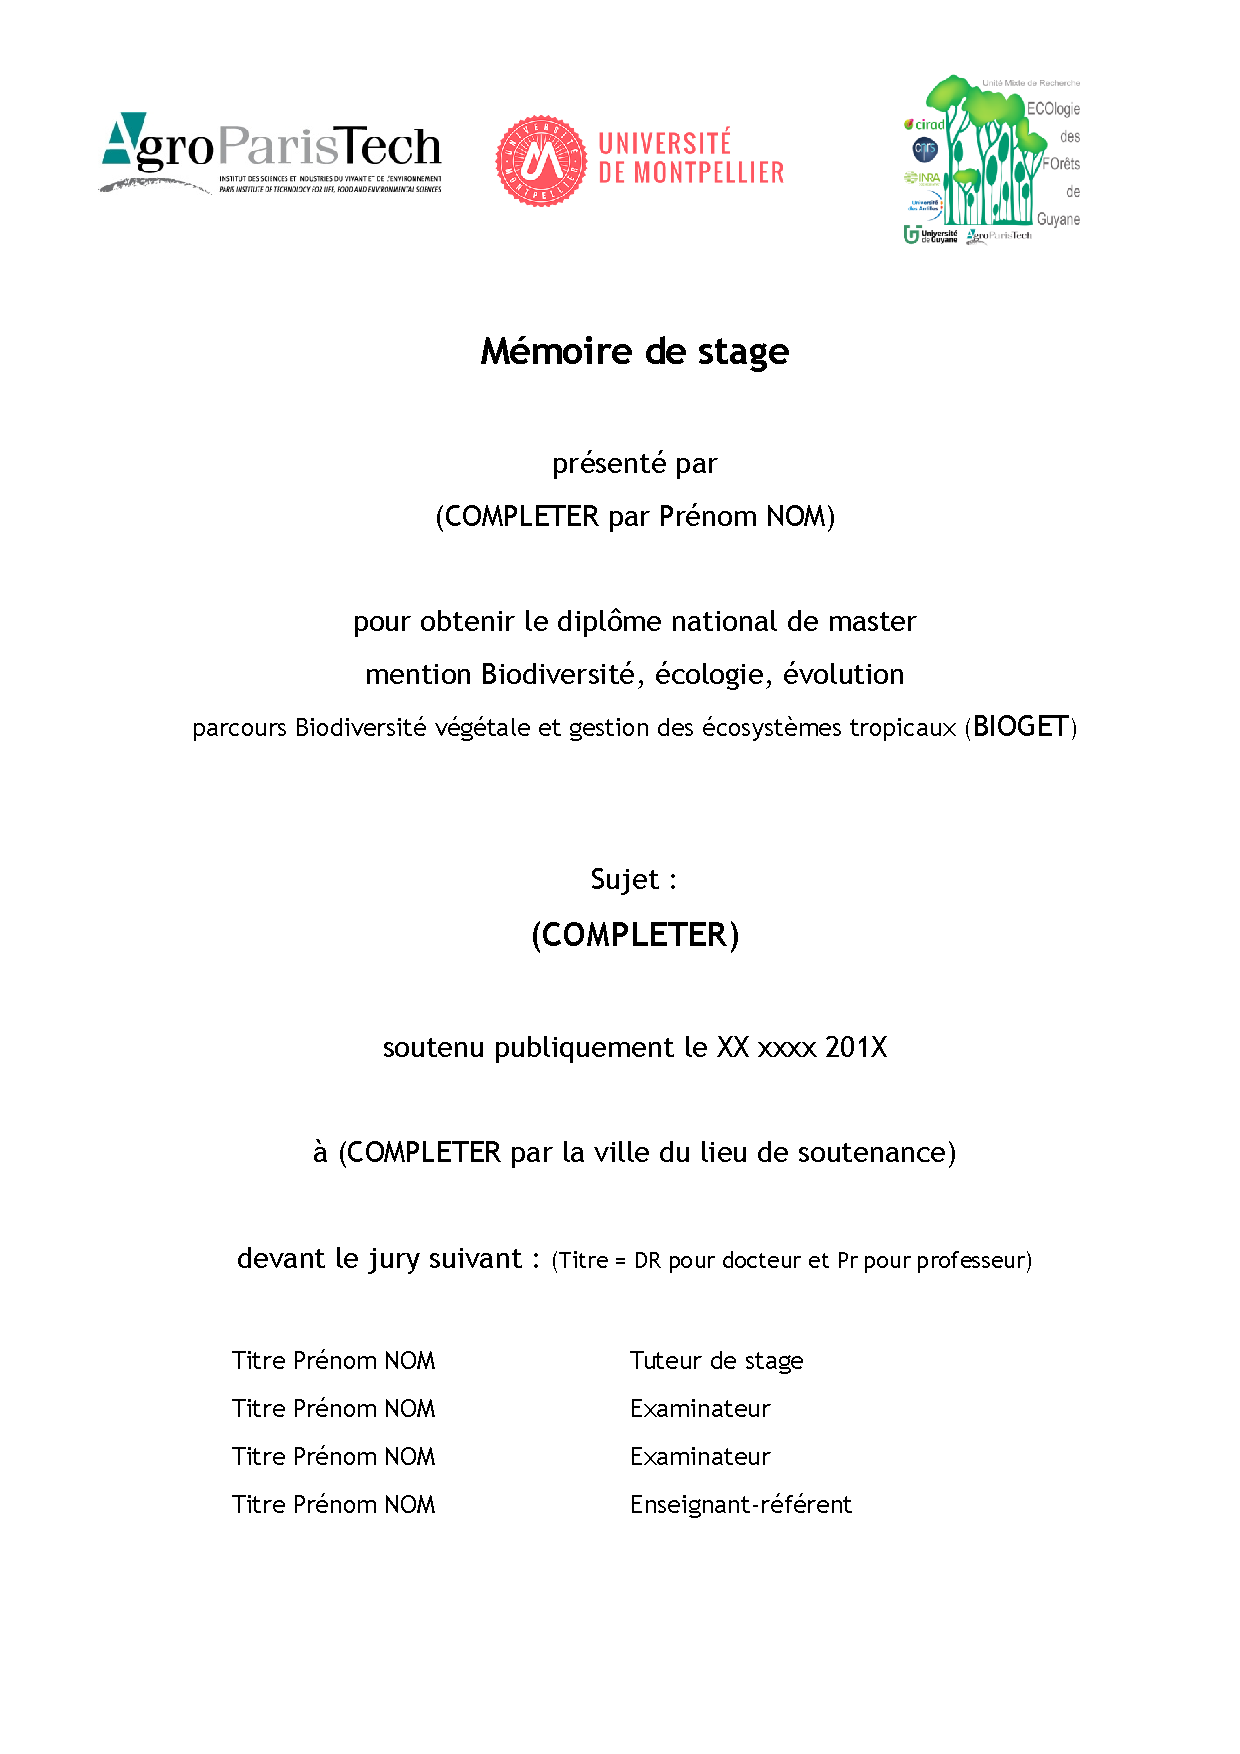
\includegraphics{images/main.pdf}
\end{center}

\setlength{\abovedisplayskip}{-5pt}
\setlength{\abovedisplayshortskip}{-5pt}

{
\hypersetup{linkcolor=black}
\setcounter{tocdepth}{2}
\tableofcontents
}
\section*{Résumé et Abstract}\label{resume-et-abstract}
\addcontentsline{toc}{section}{Résumé et Abstract}

Écrire le résumé français ici\ldots{}

Write the english abstract here\ldots{}

\section*{Acknowledgments}\label{acknowledgments}
\addcontentsline{toc}{section}{Acknowledgments}

I would like to thank\ldots{}

\section*{Introduction}\label{introduction}
\addcontentsline{toc}{section}{Introduction}

Sutainable forest management in the tropics (i.e.~managed selective
harvesting of timber) has been widely promoted internationnaly to combat
tropical deforestation and degradation \citep{Zimmerman2012}. Currently
tropical logging accounts for one eight of global timber production
\citep{Blaser2011} and is still increasing. Most tropical timber
production originates from selective logging, the targeted harvesting of
timber from commercial species in a single cuttint cycle
\citep{Martin2015}.

On the other hand, tropical rainforests have fascinated ecologists due
to their outstanding diversity \citep{connell_diversity_1978}.
Effectively tropical forests host over half of the Earth's biodiversity
\citep{Scheffers2012}. High biodiversity from tropical rainforests is
the source of many ecosystem functions. Amongst others, tropical forests
play a key role in biogeochemical cycles, including carbone storage
\citep{Lewis2004}. \textbf{Add insights into carbon storage role of
tropical forest.} Ecosystem functions from tropical forests support
numerous ecosystem services, such as timber production and climate
regulation.

But several authors argue that selective logging represents a major
threat to biodiversity
\citep{Carreno-Rocabado2012, DeAvila2015, Gibson2013, Martin2015, Zimmerman2012},
challenging the sustainable definition from current selective logging.
We consequently need to assess both short and long term impacts of
selective logging on tropical forest ecosystems to implement better
syslvicultural practives in order to reach sustainability.

The question of selective logging impact on tropical forest can be
directly related to the emerging field of biodiversity and ecosystem
functionning \citep{Loreau2000}. Tropical forest outstanding
biodiversity will be both a factor and a result of forest ecosystem
response to logging disturbance. And forest ecosystem response to
logging disturbance will directly modify ecosystem functionning in both
short and long term. Consequently assessing selective logging effect on
tropical forest linking biodiversity and ecosystem seems an obvious and
promising way \citep{Loreau2010}. \textbf{Paragraph to fully review !}

Negative short term impacts of selective logging have been assessed
\citetext{\citealp{Carreno-Rocabado2012}; \citealp{DeAvila2015}; \citealp[but
see][]{Martin2015}}. Much less is known about the long term impact
\citep{Osazuwa-Peters2015}. The main reason is the difficulty to conduct
long term empirical study \citep[but see][]{Herault2010}, which can be
completed by the use of forest simulators
\citep{Huth2004, Khler2004, Ruger2008, Tietjen2006}. Individual-based
models of forest dynamics present the perfect framework to develop such
joint biodiversity-ecosystem approaches \citep{Li}. Individual-based
models describe forest `patches' accumulating carbon through time,
assessing tree growth within the patch, or releasing carbon through gap
opening \citep{Bugmann2001}. Up to several dozens of different Plant
Functional Types (PFTs) are generally defined and models can sometimes
be fully spatially explicit \citep{Pacala1996}. Recently, the forest
growth simulator TROLL \citep{Chave1999}, an individual-based and
spatially explicit forest model, was developped to introduce recent
advances in plant physiological community. TROLL model relates
physiological processes to species-specific functional traits
\citep{Li}. Consequently, TROLL model allow to simulate fully a
neotropical forest biodiversity to study biodiversity-ecosystem
functionning link response to logging disturbance.

\textbf{Major question greater diversity (taxonomic and functional)
brought a better resilience to disturbance ?}

\section{Model description}\label{model-description}

\subsection{Overview}\label{overview}

TROLL model each tree indivdually in a located environment. Thus TROLL
model, alongside with SORTIE \citep{Pacala1996, Uriarte2009} and FORMIND
\citep{Fischer2016, Kohler1998}, can be defined as an individual-based
and spatially explicit forest growth model. TROLL simulates the life
cycle of individual trees from recruitment, with a diameter at breast
height (dbh) above 1 cm, to death with growth and seed production. Trees
are growing in a located light environment explicitly computed witin
voxels of 1 \(m^3\). Each tree is consistently defined by its age,
diameter at brest height (dbh), height (h), crown radius (CR), crown
depth (CD) and leaf area (LA) (see figure \ref{fig:TROLLtree}). Tree
geometry is calculated with allometric equations but leaf area vary
dinamically within each crown following carbon allocations. Voxels
resolution of 1 \(m^3\) allow the establishment of maximum one tree by
1x1 m pixels. Each tree is flagged with a species label inherited from
the parent tree through the seedling recruitment. A species label is
associated to a number of species specific parameters (see table
\ref{tab:traits}) related to functional trait values which can be
sampled on the field.

\begin{table}

\caption{\label{tab:traits}Species-specific parameters used in TROLL from @Li. Data originates from the BRIDGE [@Baraloto2010] and TRY [@Kattge2011] datasets.}
\centering
\begin{tabular}[t]{l|l|l}
\hline
Abbreviation & Description & Units\\
\hline
\$LMA\$ & leaf mass per area & \$g.m\textasciicircum{}-2\$\\
\hline
\$N\_m\$ & leaf nitrogen content per dry mass & \$mg.g\textasciicircum{}-1\$\\
\hline
\$P\_m\$ & leaf phosphorous content per dry mass & \$mg.g\textasciicircum{}-1\$\\
\hline
\$wsg\$ & wood specific gravity & \$g.cm\textasciicircum{}-3\$\\
\hline
\$dbh\_\{thresh\}\$ & diameter at breasth height threshold & \$m\$\\
\hline
\$h\_\{lim\}\$ & asymptotic height & \$m\$\\
\hline
\$a\_h\$ & parameter of the tree-height-dbh allometry & \$m\$\\
\hline
\end{tabular}
\end{table}

Carbon assimilation is computed over half-hourly period of a
representative day. Then allocation is computed to simulate tree growth
from an explicit carbone balance (in contrast to previous models).
Finally environment is updated at each timestep set to one month.
Seedlings are not simulated explicitly but as a pool. In addition
belowground processes, herbaceous plants, epiphytes and lianas are not
simulated inside TROLL. The source code is written in C++ and available
upon request. All analyses were conducted in R version 3.4.0
\textbf{Cite R, add entry in Mendeley}.

\begin{figure}[htbp]
\centering
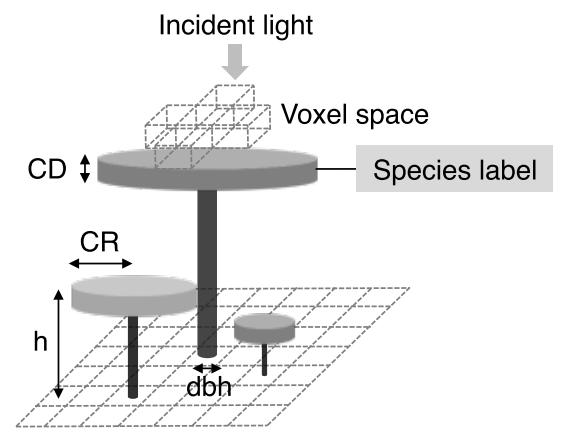
\includegraphics{images/TROLLtree.png}
\caption{\label{fig:TROLLtree}Individuals tree inside TROLL explicit spatial
grid from \citet{Li}. Tree geometry (crown radius CR, crown depth CD,
height h, diameter at breast height dbh) is updated at each timestep
following allometric relationship with assimilated carbon allocated to
growth. Each tree is flagged with a species label linking to its
species-specific attributes. Light is compputed explicitly at each
timestep for each voxel.}
\end{figure}

\subsection{Abiotic environment}\label{abiotic-environment}

A voxel space, with a resolution of 1 \(m^3\), is used to explicilty
model the abiotic environment. For each tree crown, leaf area density is
calculated on tree geometry assuming a uniform distriution across voxels
occupied by the crown. Leaf area density is computed within each voxel
summing all tree crowns inside the voxel \(v\), and is denoted
\(LAD(v)\) (leaf area per voxel in \(m².m^-3\)). The vertical sum of
\(LAD\) from voxel \(v\) to the ground level defines \(LAI(v)\) (leaf
area per fround area in \(m^2.m^-2\) commonly called leaf area index):

\begin{equation}
  LAI(v) = \sum _{v'=v} ^\infty LAD(v') 
  \label{eq:LAI}
\end{equation}

Daily variations in light intensity (photosynthetic photon flux density
PPFD in \(\mu mol_{photons}.m^-2.s^-1\)), temperature (T in degrees
Celsius), and vapor pressure deficit (VPD in \(kPA\)) are computed to
assess carbon assimilation within each voxel of the canopy and for a
representative day per month (see Appendix 1 from \citet{Li} for further
details). Variation of PPFD Within the canopy is calculated as a loacal
Beer-Lambert extinction law:

\begin{equation}
  PPFD_{max,month}(v) = PPFD_{top,max,month}*e^{-k*LAI(v)}
  \label{eq:PPFD}
\end{equation}

The daily maximum incident PPFD at the top of canopy
\(PPFD_{top,max,month}\) is given as input. The extinction rate \(k\) is
assumed as constant (see table \ref{tab:par} for parameters value),
besides is variation with zenith angle and species leaf inclination
angle \citep{Meir2000}. Moreover only vertical light diffusion is
considered ignoring lateral light diffusion, which can have an important
role especially in logging gaps. Finally, intra-day variation at half
hour time steps \(t\) for a representative day every month are used to
compute \(PPFD_{month}(v,t)\), \(T_{month}(v,t)\) and
\(VPD_{month}(v,t)\). Water and nutrient process both in soil and inside
trees are not simulated.

\subsection{Photosynthesis}\label{photosynthesis}

\subsection{Autotrophic respiration}\label{autotrophic-respiration}

\subsection{Carbon uptake}\label{carbon-uptake}

\subsection{Tree growth}\label{tree-growth}

\subsection{Recruitment}\label{recruitment}

\subsection{Mortality}\label{mortality}

\section{Sensitivity analysis}\label{sensitivity-analysis}

\subsection{Functional traits}\label{functional-traits}

\subsection{Seed rain}\label{seed-rain}

\section{Disturbance}\label{disturbance}

\subsection{Model description}\label{model-description-1}

\subsection{Design of experiment}\label{design-of-experiment}

\begin{figure}[htbp]
\centering
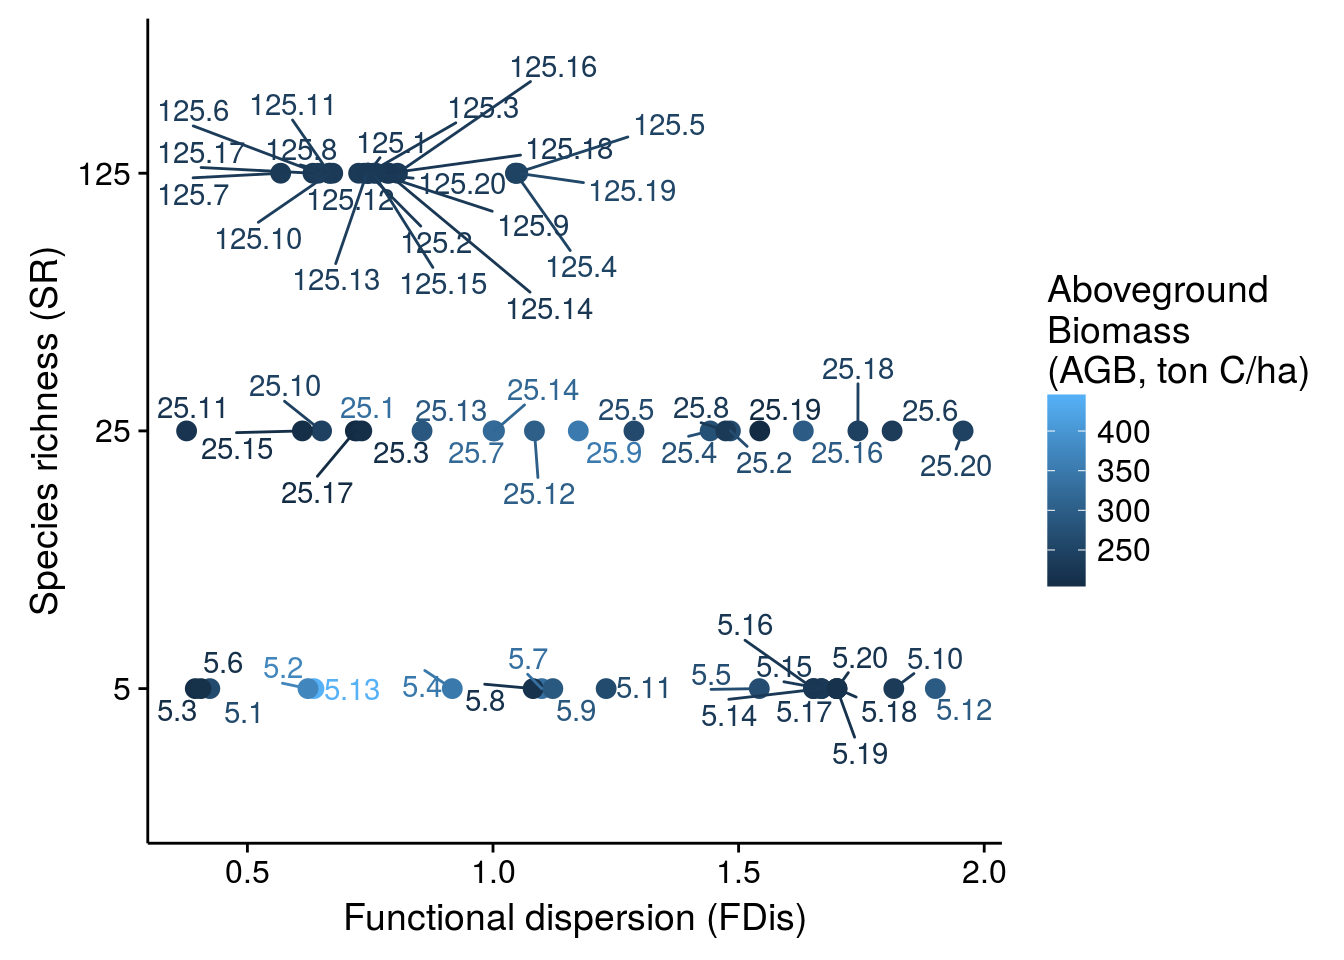
\includegraphics{master-thesis_files/figure-latex/DOE-1.pdf}
\caption{\label{fig:DOE}Experimental design before disturbance. Communities
are implemented along a gradient of species richness (SR) and functional
dispersion (FDis) resulting in a broad range of aboveground biomass
(AGB). FDis was caluclated based on 4 functional traits (leaf mass per
area, wood specific gravity, maximum diameter, maximum height).}
\end{figure}

\subsection{Outputs anlaysis ?}\label{outputs-anlaysis}

\subsubsection{Resistance and resilience
metrics}\label{resistance-and-resilience-metrics}

\subsubsection{Biodiversity
partitioning}\label{biodiversity-partitioning}

\section{Selective logging}\label{selective-logging}

\subsection{Model description}\label{model-description-2}

\subsubsection{Designation}\label{designation}

\subsubsection{Selection}\label{selection}

\subsubsection{Rotten trees}\label{rotten-trees}

\subsubsection{Felling}\label{felling}

\subsubsection{Tracks}\label{tracks}

\subsubsection{Gap damages}\label{gap-damages}

\subsection{Design of experiment}\label{design-of-experiment-1}

\subsection{Outputs analysis ?}\label{outputs-analysis}

\subsubsection{Resistance and resilience
metrics}\label{resistance-and-resilience-metrics-1}

\subsubsection{Biodiversity
partitioning}\label{biodiversity-partitioning-1}

\section{Results}\label{results}

\section{Discussion}\label{discussion}

\bibliography{/home/sylvain/Documents/Bibliography/library.bib}


\end{document}
